\chapter{Appendix}
\section{Distributions}
\subsection{Matrix Generalized Inverse Gaussian}
The Matrix \gls{MGIG} distribution is a probability distribution over positive definite symmetric ($pxp$) matrices $\{X:X>0\}$ \citet{butler_generalized_1998}.
It has recently been shown to be unimodal \citep{fazayeli2016matrix}.

\subsubsection{Butler Parameterization}
\label{MGIG_BUTLER}
In the models we mostly denote the \gls{MGIG} by the parametrization of \citet{butler_generalized_1998}
as it is the most commonly used one.
\begin{equation}
\matr{X} \sim \mathcal{MGIG}_{B}(\lambda, \matr{A}, \matr{B}) 
\end{equation}
\begin{equation*}
p(\matr{X}) \propto \det(\matr{X})^{\lambda - \frac{1}{2}(p+1)}
\exp \tr
\Big(
	-\frac{1}{2} (\matr{A}\matr{X} + \matr{B} \matr{X}^{-1} )
\Big)
\end{equation*}

\subsubsection{Letac Parameterization}
\label{MGIG_LETAC}
For sampling from the \gls{MGIG}, we use a notation similar to the one used for the \gls{GIG} in \cite{letac1983characterization}.
\begin{equation}
\matr{X} \sim \mathcal{MGIG}_{L}(n', \matr{A}, \matr{B}) 
\end{equation}
\begin{equation*}
p(\matr{X}) \propto \det(\matr{X})^{-n' - 1}
\exp \tr
\Big(
-\frac{1}{2} (\matr{A}\matr{X} + \matr{B} \matr{X}^{-1} )
\Big)
\qquad
n'>\frac{p-1}{2}
\end{equation*}

\section{Model}
\label{A:model}
\begin{math}
\\
\begin{array}{lclr}
\matr{x}_{1,\dots,n} &\overset{iid}{\sim}& \mathcal{N}_{(p+q)}(0, \matr{\Sigma})
\\
\matr{X}&=&(\bm{x}_1,\dots,\bm{x}_n)  & \matr{X}\in \mathbb{R}^{(p+q)\times n}
%\quad
\\ \\
\matr{S} &=& \matr{X} \matr{X}^T
\\
\matr{S} &\sim& \mathcal{W}_{p+q}(n, \matr{\Sigma})
\end{array}
\end{math}
\\
\\
\begin{equation*}
\matr{\Sigma^{-1}} = \matr{W}=
\raisebox{0.3\baselineskip}{$
	\begin{blockarray}{ccc}
	p & q& \\
	\begin{block}{(cc)l}
		\matr{W}_{11} & \matr{W}_{12}&p \\
		\matr{W}_{12}^T & \matr{W}_{22}&q \\
	\end{block}
	\end{blockarray}
$}
\quad \quad \quad \quad 
\matr{S}=
\raisebox{0.3\baselineskip}{$
	\begin{blockarray}{ccc}
	p & q& \\
	\begin{block}{(cc)l}
	\matr{S}_{11} & \matr{S}_{12}&p \\
	\matr{S}_{12}^T & \matr{S}_{22}&q \\
	\end{block}
	\end{blockarray}
	$}
\end{equation*}
\\ \\
Let 
$$\matr{W}_{22.1} = \matr{W}_{22} - \matr{W}_{12}^T \matr{W}_{11}^{-1} \matr{W}_{12}$$
be the Schur complement of $\matr{W}_{22}$.


\subsection{Likelihood}

\begin{align*}
p(\matr{S}|\matr{W}) &\propto \det(\matr{W})^{\frac{n}{2}} det(\matr{S})^{\frac{n-(p+q)-1}{2} }\exp \tr \big( - \frac{1}{2} \matr{W} \matr{S}\big)
\end{align*}

\subsection{Prior}
\begin{align*}
P(\matr{W}|\matr{T}) &=
\mathcal{W}_{p+q} \big(p + q + 1, \matr{I}\big) p(\matr{W}_{12} | \matr{T} )
\\
&\propto \exp\tr \Big(-\frac{1}{2} \matr{W}\Big)
\prod_{{\substack{i=1,\dots,p\\j=1,\dots,q}} }   \frac{1}{\sqrt{2\pi \matr{T}_{ij}}} \exp 
\Big( - \frac{(\matr{W}_{12})_{ij}^2}{2\matr{T}_{ij}} \Big) 
\\ \\
P(\matr{T}| \lambda) &\propto
\prod_{{\substack{i=1,\dots,p\\j=1,\dots,q}} }   \frac{\lambda^2}{2} \exp \Big( - \frac{\lambda^2}{2} \matr{T}_{ij} \Big)
\end{align*}
\subsection{Joint Distribution}
\begin{align*}
p(\matr{W}, \matr{S}, \matr{T} | \lambda) =& p(\matr{W}_{11}, \matr{W}_{12}, \matr{W}_{22}, \matr{S}, \matr{T} | \lambda) \\
\propto& \quad \det(\matr{W})^\frac{n}{2} 
\det(\matr{S})^{\frac{n-(p+q)-1}{2} }
\\
&\times \exp \tr \big( - \frac{1}{2} \matr{W} \matr{S}\big)		
 \exp\tr \Big(-\frac{1}{2} \matr{W}\Big)
\\
&\times \prod_{{\substack{i=1,\dots,p\\j=1,\dots,q}} }  \frac{1}{\sqrt{2\pi \matr{T}_{ij}}} \exp 
\Big( - \frac{(\matr{W}_{12})_{ij}^2}{2\matr{T}_{ij}} \Big) 
\\
&\times \prod_{{\substack{i=1,\dots,p\\j=1,\dots,q}} } \frac{\lambda^2}{2} \exp \Big( - \frac{\lambda^2}{2} \matr{T}_{ij} \Big)
\\\\
= &\det(\matr{W})^{\frac{n}{2}}  \det(\matr{S})^{\frac{n-(p+q)-1}{2}} 
\\
&\exp\Bigg(-\frac{1}{2} \tr [\matr{WS}+\matr{W}] - \frac{1}{2} \sum_{{\substack{i=1,\dots,p\\j=1,\dots,q}} } \frac{(\matr{W}_{12})_{ij}^2}{\matr{T}_{ij}}  \Bigg) 
\\
&\times \Big[\prod_{{\substack{i=1,\dots,p\\j=1,\dots,q}} }  \frac{1}{\sqrt{2\pi \matr{T}_{ij}}}\Big]
p(\matr{T}|\lambda)
\end{align*}
\subsubsection{Reparametrization with $\matr{W}_{11}, \matr{W}_{12}, \matr{W}_{22.1}$}
$$ J\big((\matr{W}_{11}, \matr{W}_{12}, \matr{W}_{22}) \rightarrow (\matr{W}_{11}, \matr{W}_{12}, \matr{W}_{22.1})\big) = \matr{1} $$
\begin{align*}
\det(\matr{W}) &= \det(\matr{W}_{11}) \det(\matr{W}_{22} - \matr{W}_{12}^T \matr{W}_{11}^{-1}\matr{W}_{12})
\\
&= \det(\matr{W}_{11}) \det(\matr{W}_{22.1})
\\
\\
\tr(\matr{WS}) &= \tr\big[\matr{W}_{11}\matr{S}_{11} + \matr{W}_{12}\matr{S}_{21} + \matr{W}_{21}\matr{S}_{12} + \matr{W}_{22}\matr{S}_{22}   \big]
\\
&= \tr\big[\matr{W}_{11}\matr{S}_{11} + \matr{W}_{12}\matr{S}_{12}^T + \matr{W}_{12}^T\matr{S}_{12} + (\matr{W}_{22.1} + \matr{W}_{12}^T\matr{W}_{11}^{-1}\matr{W}_{12}) \matr{S}_{22}   \big]
\\
&= \tr\big[
\Cline[blue]{\matr{W}_{11}\matr{S}_{11}} + 
\Cline[yellow]{\matr{W}_{12}\matr{S}_{12}^T + 
	\matr{W}_{12}^T\matr{S}_{12}} + 
\Cline[red]{\matr{W}_{22.1}\matr{S}_{22}} + 
\Cline[green]{\matr{W}_{12}^T\matr{W}_{11}^{-1}\matr{W}_{12}\matr{S}_{22}}   
\big]
\\
\\
\tr(\matr{W}) &= \tr(\matr{W}_{11}) + \tr(\matr{W}_{22})
\\
&= \tr(\Cline[blue]{\matr{W}_{11}}) + 
\tr(\Cline[red]{\matr{W}_{22.1}}) +
\tr(\Cline[green]{\matr{W}_{12}^T\matr{W}_{11}^{-1}\matr{W}_{12}})
\end{align*}

\begin{align*}
p(\matr{W}_{11}, \matr{W}_{12}, &\matr{W}_{22.1}, \matr{S}, \matr{T} | \lambda) \propto
\\
&\det(\matr{W}_{11})^{n/2} \det(\matr{W}_{22.1})^{n/2} \det(\matr{\matr{S}})^{\frac{n-(p+q)-1}{2}}
\\
\times& \exp \Big(
-\frac{1}{2}
\tr\big[
\Cline[blue]{\matr{W}_{11} (\matr{S}_{11} + \matr{I}) }+ 
\Cline[red]{\matr{W}_{22.1}  (\matr{S}_{22} + \matr{I})} + 
\\
&\quad \quad \quad \quad \quad \quad
\Cline[yellow]{2 (\matr{W}_{12}^T\matr{S}_{12})} +
\Cline[green]{
	\matr{W}_{12}^T \matr{W}_{11}^{-1}\matr{W}_{12} 
	(\matr{S}_{22} + \matr{I})}
\big]
\Big)
\\
\times& \exp\Big(- \frac{1}{2} \sum_{{\substack{i=1,\dots,p\\j=1,\dots,q}} } \frac{(\matr{W}_{12})_{ij}^2}{\matr{T}_{ij}} \Big) \quad \Big[\prod_{{\substack{i=1,\dots,p\\j=1,\dots,q}} }  \frac{1}{\sqrt{2\pi \matr{T}_{ij}}}\Big]
\quad
p(\matr{T}|\lambda)
\end{align*}

\subsection{Full Posterior}
Let $\matr{D} = \text{diag}(\text{vec}(\matr{T}))^{-1}$, i.e. a diagonal matrix, where the elements are the inverses of the elements of $\matr{T}$

\begin{align*}
\exp\Big(- \frac{1}{2}  \sum_{{\substack{i=1,\dots,p\\j=1,\dots,q}} } \frac{(\matr{W}_{12})_{ij}^2}{\matr{T}_{ij}} \Big)
&= 
\exp \Big(
-\frac{1}{2} \Cline[gray]{\text{vec}(\matr{W}_{12})^T\  \matr{D} \ \text{vec}(\matr{W}_{12})
}
\Big)
\\
\\
\tr(\Cline[yellow]{\matr{W}_{12}^T \matr{S}_{12}})  &= \text{vec}(\matr{W}_{12})^T \text{vec}(\matr{S}_{12})
\end{align*}


\begin{align}
p(\matr{W}_{11}, \matr{W}_{12}, \matr{W}_{22.1}, \matr{T} | \matr{S}, \lambda) \propto 
&\det(\matr{W}_{11})^{n/2} \exp \Big( - \frac{1}{2} \tr\big[ \Cline[blue]{\matr{W}_{11} (\matr{S}_{11} + \matr{I}) }\big]\Big)
\label{joint_1}\\
&\times \det(\matr{W}_{22.1})^{n/2} \exp \Big( - \frac{1}{2} \tr\big[ \Cline[red]{\matr{W}_{22.1}  (\matr{S}_{22} + \matr{I})}\big]\Big)
\nonumber\\
&\times \exp\Big(
-\frac{1}{2} \tr \big[ \Cline[green]{\matr{W}_{12}^T\matr{W}_{11}^{-1}\matr{W}_{12}\big(\matr{S}_{22}+\matr{I}\big)}   \big]
\Big)
\nonumber\\
&\times \exp \Big(
-\frac{1}{2} 
\Cline[gray]{
	\text{vec}(\matr{W}_{12})^T\  \matr{D} \ \text{vec}(\matr{W}_{12})
}
\Big)
\nonumber\\
&\times \exp \Big( 
\Cline[yellow]{
	-\text{vec}(\matr{W}_{12})^T \text{vec}(\matr{S}_{12})\Big)
}
\nonumber\\
&\times \Big[\prod_{{\substack{i=1,\dots,p\\j=1,\dots,q}} }  \frac{1}{\sqrt{2\pi \matr{T}_{ij}}}\Big]
p(\matr{T} | \lambda)
\nonumber\\\nonumber \\
\nonumber\\
\tr \Big[ \Cline[green]{\matr{W}_{12}^T \matr{W}_{11}^{-1}\matr{W}_{12}(\matr{S}_{22}+\matr{I})}\Big]
&= \text{vec}(\matr{W}_{12})^T \text{vec}(\matr{W}_{11}^{-1} \matr{W}_{12}(\matr{S}_{22} + \matr{I} ))
\nonumber\\
&\overset{\text{\tiny{(520 Matr. Cookbook)}}}{=}
\text{vec}(\matr{W}_{12})^T \Big[
(\matr{S}_{22} + \matr{I})^T \otimes \matr{W}_{11}^{-1} \Big]
\text{vec}(\matr{W}_{12})
\nonumber\\
&= \text{vec}(\matr{W}_{12})^T \Big[
(\matr{S}_{22} + \matr{I}) \otimes \matr{W}_{11}^{-1} \Big]
\text{vec}(\matr{W}_{12})
\nonumber\\
\nonumber\\  \nonumber\\
p(\matr{W}_{11}, \matr{W}_{12}, \matr{W}_{22.1}, \matr{T} | \matr{S}, \lambda) \propto&
\det(\matr{W}_{11})^{n/2} \exp \Big( - \frac{1}{2} \tr\big[ \matr{W}_{11} (\matr{S}_{11} + \matr{I}) \big]\Big)
\label{joint_2}\\
&\times \det(\matr{W}_{22.1})^{n/2} \exp \Big( - \frac{1}{2} \tr\big[\matr{W}_{22.1}  (\matr{S}_{22} + \matr{I})\big]\Big)
\nonumber\\
&\times \exp\Big(
-\frac{1}{2}\Cline[gray]{\Cline[green]{\text{vec}(\matr{W}_{12})^T \Big[
		(\matr{S}_{22} + \matr{I}) \otimes \matr{W}_{11}^{-1} +\matr{D}\Big]
		\text{vec}(\matr{W}_{12})}}
- \text{vec}(\matr{W}_{12})^T \text{vec}(\matr{S}_{12})
\Big)
\nonumber\\
&\times \Big[\prod_{{\substack{i=1,\dots,p\\j=1,\dots,q}} }  \frac{1}{\sqrt{2\pi \matr{T}_{ij}}}\Big]
p(\matr{T}|\lambda)
\nonumber
\end{align}
\subsubsection{Factorization of the Posterior}
\label{A:factorized_post}
We can now factorize wrt. $W_{22.1}$.
$$ p(\matr{W}_{11}, \matr{W}_{12}, \matr{W}_{22.1}, \matr{T} | \matr{S}, \lambda)
= p(\matr{W}_{11}, \matr{W}_{12}, \matr{T} | \matr{S}, \lambda) p(\matr{W}_{22.1} | \matr{S}, \lambda) 
$$

Using
\begin{align*}
\det(\matr{S})^{\frac{n-(p+q)-1}{2}} &= \det(\Syy)^{\frac{n-p-q-1}{2}} \det(\Sxxs)^{\frac{n-p-q-1}{2}}
\\
&=
\det(\Syy)^{\frac{n-p-2q-1}{2}}\det(\Syy^{-1})^{-\frac{q}{2}} \det(\Sxxs)^{\frac{n-p-q-1}{2}}
\end{align*}
It follows that

\begin{align}
\label{A:W221}
p(\Wyys|\matr{S}, \lambda)
\propto 
\det(\Syy)^{\frac{n-p-q-1}{2}}
\det(\Wyys)^{\frac{n}{2}}
\exp\big(
	-\frac{1}{2} \tr \big[
		\Wyys (\Syy+\matr{I})
	\big]
\big)
\end{align}
Comparing the determinants of \autoref{A:W221} to the ones from the Wishart (denoted by $df$, furthermore we know the size of the Wishart distributed matrix is $q$):
\begin{align*}
\det(\Wyys)^{\frac{df-q-1}{2}} &= \det(\Wyys)^{\frac{n}{2}}
\\
\det(\Syy)^{\frac{df}{2}} &= \det(\Syy)^{\frac{n-p-2q-1}{2}}
\end{align*}
\begin{align*}
\Rightarrow&
q = df - n - 1
\\
&df = n -p-2q-1
\\
&\quad= n-p-2(df-n-1)-1
\\
\Rightarrow&
3df = 3n - p + 1
\\
\Rightarrow&
df = n- \frac{(p-1)}{3}
\end{align*}
$$\Downarrow$$
\begin{equation}
\boxed{
	\Wyys|\matr{S}, \lambda \sim \mathcal{W}\Big(n-\frac{(p-1)}{3}, \Syy \Big)
	}
\end{equation}
\\
\\

Additionally, now the joint posterior for $(\Wxx, \Wxy)$ is:
\begin{align}
p(\matr{W}_{11}, \matr{W}_{12}, \matr{T} | \matr{S}, \lambda)
\propto& \quad
\det(\matr{W}_{11})^{n/2} \exp \Big( - \frac{1}{2} \tr\big[ \matr{W}_{11} (\matr{S}_{11} + \matr{I}) \big]\Big)
\label{marginal_joint}\\
&\times \exp\Big(
-\frac{1}{2}\text{vec}(\matr{W}_{12})^T \Big[
(\matr{S}_{22} + \matr{I}) \otimes \matr{W}_{11}^{-1} +\matr{D}\Big]
\text{vec}(\matr{W}_{12})
- \text{vec}(\matr{W}_{12})^T \text{vec}(\matr{S}_{12})
\Big)
\nonumber \\
&\times \Big[\prod_{{\substack{i=1,\dots,p\\j=1,\dots,q}} }  \frac{1}{\sqrt{2\pi \matr{T}_{ij}}}\Big]
p(\matr{T}|\lambda)
\nonumber
\end{align}
\subsection{Posterior Conditionals}
\label{A:post_cond}
\subsubsection{$\matr{W}_{12}$}
We condition \autoref{marginal_joint} additionally on $\matr{T}$ and $\matr{W}_{11}$:

\begin{align*}
p(\matr{W}_{12} | \matr{W}_{11}, \matr{T}, \matr{S}, \lambda)
&\propto 
\exp\Big(
-\frac{1}{2}\text{vec}(\matr{W}_{12})^T \Big[
(\matr{S}_{22} + \matr{I}) \otimes \matr{W}_{11}^{-1} +\matr{D}\Big]
\text{vec}(\matr{W}_{12})
- \text{vec}(\matr{W}_{12})^T \text{vec}(\matr{S}_{12})
\Big)
\\
&=\exp\Big(-\frac{1}{2} x^T\matr{C}x - b^Tx\Big) 
\\
&\overset{\text{\tiny{(8.16Matr. Cookbook)}}}{=}
\exp \Big(-\frac{1}{2} (x+\matr{C}^{-1}b)^T\matr{C}(x+\matr{C}^{-1}b) + \frac{1}{2}b^T\matr{C}^{-1}b\Big)
\end{align*}

with 
$$
x = \text{vec}(\matr{W}_{12})
\quad \quad \quad
\matr{C} = \Big[
(\matr{S}_{22} + \matr{I}) \otimes \matr{W}_{11}^{-1} +\matr{D}\Big]
\quad \quad \quad
b = \text{vec}(\matr{S}_{12})
$$
$$\Downarrow$$
\begin{equation}
	\boxed{
		\text{vec}(\matr{W}_{12}) | \matr{W}_{11}, \matr{T}, \matr{S}, \lambda \sim \mathcal{N}(-\matr{C}^{-1} \text{vec}(\matr{S}_{12}), \matr{C}^{-1})
	}
\end{equation}

\subsubsection{$\matr{W}_{11}$}
We take \autoref{joint_1}, marginalize wrt. $\matr{W}_{22.1}$ and then additionally condition on $ \matr{W}_{12}, \matr{T}$:

\begin{align*}
p(\matr{W}_{11} | \matr{W}_{12}, \matr{T}, \matr{S}, \lambda)
& \propto
\det(\matr{W}_{11})^{n/2}
\exp \Big(
-\frac{1}{2} \tr\big[
\matr{W}_{11}(\matr{S}_{11}+ \matr{I}) + \matr{W}_{12}(\matr{S}_{22}+\matr{I})\matr{W}_{12}^T \matr{W}_{11}^{-1}
\big]
\Big)
\\
&=
\det(\matr{W}_{11})^{n/2}
\exp \Big(
-\frac{1}{2} \tr\big[
\underbrace{(\matr{S}_{11}+ \matr{I})}_{\text{MGIG A}} \matr{W}_{11}+ \underbrace{\matr{W}_{12}(\matr{S}_{22}+\matr{I})\matr{W}_{12}^T}_{\text{MGIG B}}\matr{W}_{11}^{-1}
\big]
\Big)
\end{align*}
$$\Downarrow$$
Comparing the determinants to the (Butler) \gls{MGIG} defined in \autoref{MGIG_BUTLER} leads to
\begin{equation}
\label{W11_MGIG_posterior}
\boxed{
	\matr{W}_{11} | \matr{W}_{12}, \matr{T}, \matr{S}, \lambda \sim 
	\mathcal{MGIG}_B
	\Big(
		\frac{n+p+1}{2}, \ 
		\matr{S}_{11}+\matr{I},\  
		\matr{W}_{12}(\matr{S}_{22}+\matr{I})\matr{W}_{12}^T
	\Big)
}
\end{equation}

\subsubsection{$\matr{T}$}
\begin{align*}
p(\matr{T}| \matr{W}_{11}, \matr{W}_{12}, \matr{S}, \lambda) \propto& 
\prod_{{\substack{i=1,\dots,p\\j=1,\dots,q}} }   \frac{1}{\sqrt{2\pi \matr{T}_{ij}}} \exp 
\Big( - \frac{(\matr{W}_{12})_{ij}^2}{2\matr{T}_{ij}} \Big) 
\prod_{{\substack{i=1,\dots,p\\j=1,\dots,q}} }   
\frac{\lambda^2}{2} 
\exp\Big( 
- \frac{\lambda^2}{2} \matr{T}_{ij} 
\Big)
\\
\\
p(\matr{T}_{ij}| \matr{W}_{11}, \matr{W}_{12}, \matr{S}, \lambda) \propto& 
\frac{1}{\sqrt{2\pi \matr{T}_{ij}}} \exp 
\Big( - \frac{(\matr{W}_{12})_{ij}^2}{2\matr{T}_{ij}} \Big)    
\frac{\lambda^2}{2} 
\exp\Big( 
- \frac{\lambda^2}{2} \matr{T}_{ij} 
\Big)
\\
=& \frac{\lambda^2}{2} \Big(\frac{1}{2\pi \matr{T}_{ij}}\Big)^{1/2} \exp \Big(-\frac{(\matr{W}_{12})_{ij}^2}{2\matr{T}_{ij}} - \frac{\lambda^2}{2} \matr{T}_{ij}\Big)
\end{align*}
Substitute $\matr{T}_{ij}$ with $\matr{T}_{ij}^{-1}$:
$
\quad
J(\matr{T}_{ij} \rightarrow \matr{T}_{ij}^{-1}) = -\matr{T}_{ij}^{-2}
$

\begin{align*}
p\Big(\frac{1}{\matr{T}_{ij}}\Big) \propto&
 -\matr{T}_{ij}^{-2} \frac{\lambda^2}{2}
\Big(
	\frac{1}{2\pi\matr{T}_{ij}^{-1}}
\Big)^{1/2} 
\exp \Big(
	- \frac{(\matr{W}_{12})_{ij}^2}{2}\matr{T}_{ij} - \frac{\lambda^2}{2}\matr{T}_{ij}^{-1}
\Big)
\\
=&
- \frac{\lambda^2}{2}
\Big(
	\frac{1}{2\pi\matr{T}_{ij}^{3}}
\Big)^{1/2} 
\exp \Big(
	- \frac{(\matr{W}_{12})_{ij}^2}{2\matr{T}_{ij}}
	\Big(
	\matr{T}_{ij}^2 - \frac{\lambda^2}{(\matr{W}_{12})_{ij}^{2}}
	\Big)
\Big)
\\
\\
&\text{Substitute }(\mu')^2 = \frac{\lambda^2}{(\matr{W}_{12})_{ij}^2}
\\
\\
=& 
- \frac{\lambda^2}{2}
\Big(
\frac{1}{2\pi\matr{T}_{ij}^{3}}
\Big)^{1/2} 
\exp \Big(
- \frac{\lambda^2}{2(\mu')^2\matr{T}_{ij}} \big(\matr{T}_{ij}^2 - 2 \matr{T}_{ij} \mu' + 2\matr{T}_{ij}\mu' + (\mu')^2 \big)
\Big)
\\
\propto& 
- \frac{\lambda^2}{2}
\Big(
\frac{1}{2\pi\matr{T}_{ij}^{3}}
\Big)^{1/2} 
\exp \Big(
- \frac{\lambda^2}{2(\mu')^2\matr{T}_{ij}} \big(\matr{T}_{ij} - \mu' \big)^2
-\frac{\lambda^2}{\mu'}
\Big)
\\
\propto&
\Big(
\frac{\lambda^2}{2\pi\matr{T}_{ij}^{3}}
\Big)^{1/2} 
\exp \Big(
- \frac{\lambda^2}{2(\mu')^2\matr{T}_{ij}} \big(\matr{T}_{ij} - \mu' \big)^2
\Big)
\end{align*}
$$\downarrow$$
\begin{equation}
\boxed{
	\matr{T}_{ij}^{-1} \sim \mathcal{IG}
	\Big(
	\mu' = \sqrt{
		\frac{\lambda^2}{(\matr{W}_{12})_{ij}^2}
	},
	\lambda' = \lambda^2
	\Big)
}
\end{equation}

\pagebreak
\section{Cooling of the posterior conditionals}

\subsection{Inverse Gaussian}
Let the Inverse Gaussian (IG) Distribution be denoted by
$$
\bm{X} \sim \mathcal{IG}(\mu, \lambda)
$$
$$
p(x) = \Big(\frac{\lambda}{2\pi x^3}\Big)^{1/2}\exp \Big[ \frac{-\lambda(x-\mu)^2}{2\mu^2 x} \Big]
$$

and the Generalized Inverse Gaussian (GIG) Distribution by
$$
\bm{Y} \sim \mathcal{GIG}(a, b, p)
$$
$$
p(y) = \frac{(a/b)^{p/2}}{2K_p(\sqrt{ab})} y^{(p-1)} \exp\Big[-\frac{1}{2}\big(ay + \frac{b}{y}\big)\Big]
$$

We can write the $\mathcal{IG}$ distribution as a special case of the $\mathcal{GIG}$ distribution:
\\
With  
\begin{equation}
\bm{Y} \sim \mathcal{GIG}(a=\frac{\lambda}{\mu^2}, b=\lambda, p=-\frac{1}{2})
\label{IG_as_GIG}
\end{equation}
we get
$$p(x\geq\bm{X}) = p(x\geq\bm{Y})$$

As a consequence, we can write the cooled $\mathcal{IG}$ in terms of the $\mathcal{GIG}$:
\begin{align*}
p(y) &\propto
y^{(p-1)} \exp\Big[-\frac{1}{2}\big(ax + \frac{b}{y}\big)\Big]
\\
\\
T &\in \mathbb{R}_{>0}
\\
p(y)^\frac{1}{T} &\propto
y^{\frac{(p-1)}{T}} \exp\Big[-\frac{1}{2T}\big(ay + \frac{b}{y}\big)\Big]
\\
&\propto 
y^{(\frac{p-1}{T}+1)-1} \exp\Big[-\frac{1}{2}\Big(\frac{a}{T}y + \frac{b/T}{y}\Big)\Big]
\\
&\propto p(z)
\end{align*}
$$
\bm{Z} \sim \mathcal{GIG}\bigg(a'=\frac{a}{T}, b'=\frac{B}{T}, p'=\Big(\frac{p-1}{T}+1\Big)\bigg)
$$
using \autoref{IG_as_GIG} we get:
\begin{equation}
\bm{Z} \sim \mathcal{GIG}\bigg(a'=\frac{\lambda/\mu^2}{T}, b'=\frac{\lambda}{T}, p'=\Big(-\frac{1.5}{T}+1\Big)\bigg)
\end{equation}


\subsection{Matrix Generalized Inverse Gaussian}
\begin{align*}
\bm{X} &\sim \mathcal{MGIG}_B(\lambda, A, B) \\
p({X}) &\propto \det({X})^{\lambda - \frac{1}{2}(p+1)}
\exp \tr
\Big(
-\frac{1}{2} (\matr{A}{X} + \matr{B} {X}^{-1} )
\Big)
\\ \\ 
T &\in \mathbb{R}_{>0}
\\
p(X)^{\frac{1}{T}}
&\propto det(X)^{\frac{{\lambda - \frac{1}{2}(p+1)}}{T}} exp \lbrack tr(-\frac{1}{2}(AX + BX^{-1} ))\rbrack^{\frac{1}{T}}
\\
&\propto det(X)^{\frac{\lambda}{T} - \frac{1}{2T}(p+1)} exp \lbrack tr(-\frac{1}{2T}(AX + BX^{-1} ))\rbrack
\\
&\propto det(X)^{\frac{\lambda}{T} - \frac{1}{2T}(p+1)} exp \lbrack tr(-\frac{1}{2}(\frac{A}{T}X + \frac{B}{T}X^{-1} ))\rbrack
\\
&\propto det(X)^{\big({\frac{\lambda}{T} - \frac{1}{2T}(p+1)} + \frac{1}{2}(p+1)\big) - \frac{1}{2}(p+1)} exp \lbrack tr(-\frac{1}{2}(\frac{A}{T}X + \frac{B}{T}X^{-1} ))\rbrack
\\
&\propto det(X)^{\big(\frac{\lambda}{T} + \frac{p+1}{2}(1-\frac{1}{T})\big) - \frac{1}{2}(p+1)} exp \lbrack tr(-\frac{1}{2}(\frac{A}{T}X + \frac{B}{T}X^{-1} ))\rbrack
\\
&\propto p(Y) 
\\
\bm{Y} &\sim \mathcal{MGIG}_B\Bigg(\Big(\frac{\lambda}{T} + \frac{p+1}{2}\big(1-\frac{1}{T}\big)\Big), \ \frac{A}{T},\ \frac{B}{T}\Bigg)
\end{align*}
\subsection{Normal Distribution}

\begin{align*}
{X} &\sim N(\mu, \Sigma)
\\
p(x) &= \big( (2\pi)^k \det{(\Sigma)}\big)^{-\frac{1}{2}} exp \lbrack - \frac{1}{2} (x-\mu)^t \Sigma^{-1} (x-\mu) \rbrack
\\ \\ 
T &\in \mathbb{R}_{>0} 
\\
p(x)^{\frac{1}{T}}&= \big( (2\pi)^k \det{(\Sigma)}\big)^{-\frac{1}{2T}} 
exp \lbrack - \frac{1}{2} (x-\mu)^t \Sigma^{-1} (x-\mu) \rbrack^{\frac{1}{T}}
\\
&\propto exp \lbrack - \frac{1}{2} (x-\mu)^t \Sigma^{-1} (x-\mu) \rbrack^{\frac{1}{T}}
\\
&\propto exp \lbrack - \frac{1}{2T} (x-\mu)^t \Sigma^{-1} (x-\mu) \rbrack
\\
&\propto exp \lbrack - \frac{1}{2} (x-\mu)^t \frac{\Sigma^{-1}}{T} (x-\mu) \rbrack
\\
&\propto exp \lbrack - \frac{1}{2} (x-\mu)^t (T \Sigma)^{-1} (x-\mu) \rbrack
\\
&\propto p(y) 
\\
Y &\sim \mathcal{N}(\mu, T \Sigma)
\end{align*}

\subsection{Wishart Distribution}
\begin{align*}
S &\sim W_p(n,\Sigma) \\
p(S) &\propto det(S)^{\frac{1}{2} (n-p-1)} etr\left(-\frac{1}{2} \Sigma^{-1} S\right) & S>0, n\geq p
\\
&\propto  det(S)^{\frac{1}{2T} (n-p-1)} etr\left(-\frac{1}{2T} \Sigma^{-1} S\right)
\\
&\propto  det(S)^{\frac{1}{2} \left( \left(\frac{n-p-1}{T} + p + 1\right) - p - 1\right)  } etr\left(-\frac{1}{2} (T\Sigma)^{-1} S\right)
\\
&\propto p(y)
\\
Y &\sim W_p\left( \frac{n-p-1}{T} + p + 1, T\Sigma\right)
\end{align*}
\pagebreak
\section{Reconstructed Graphs from Artificial Data}
In this section, multiple graphs reconstructed with the BMB and SA are shown and compared to the ground truth in terms of their graph intersection (i.e. the true positives) and the false positive predictions.
\begin{figure}
	\centering
	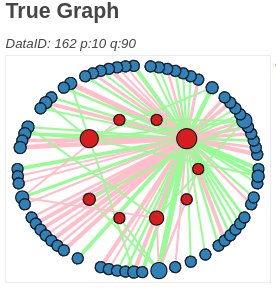
\includegraphics[width=0.3\linewidth]{graph_true_162}
	\caption{True W12 subnetwork (for artificial data set with id 162)}
	\label{fig:network_true162}
\end{figure}
\begin{figure}
	\centering
	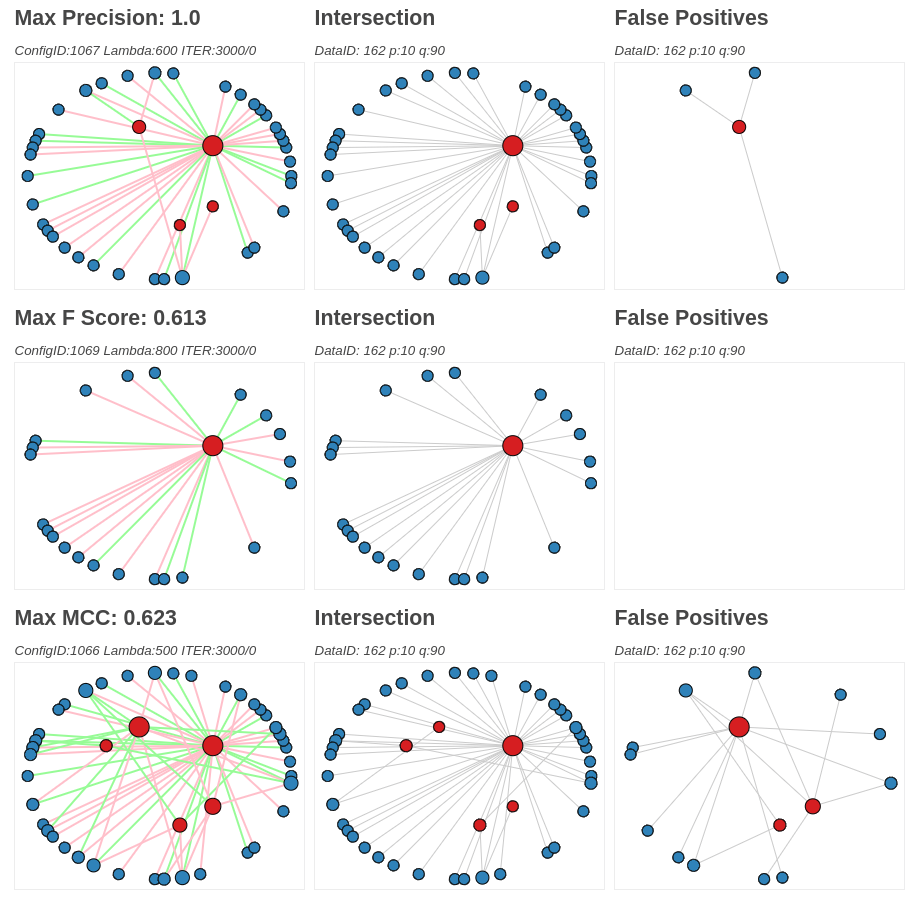
\includegraphics[width=0.9\linewidth]{graph_gibbs_162}
	\caption{W12 subnetwork reconstructed with Gibbs BMB (for artificial data set with id 162)}
	\label{fig:network_gibbs162}
\end{figure}
\begin{figure}
	\centering
	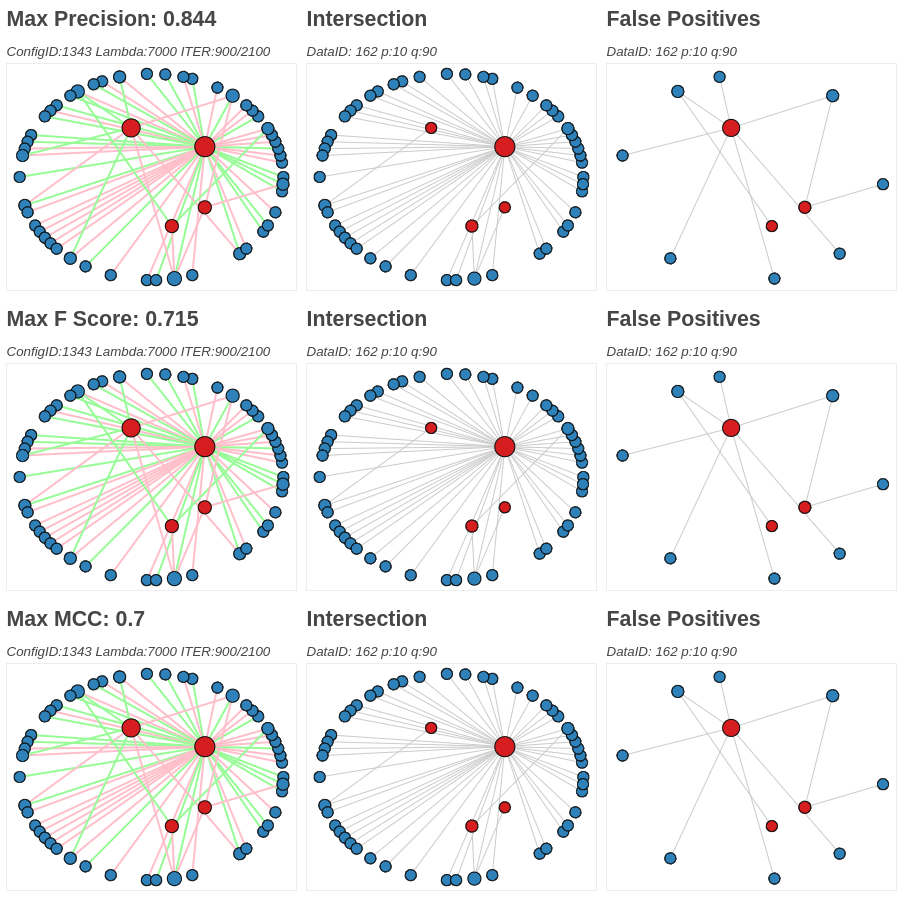
\includegraphics[width=1\linewidth]{graph_SA_162}
	\caption{W12 subnetwork reconstructed with Simulated Annealing (for artificial data set with id 162)}
	\label{fig:network_SA162}
\end{figure}
\begin{figure}
	\centering
	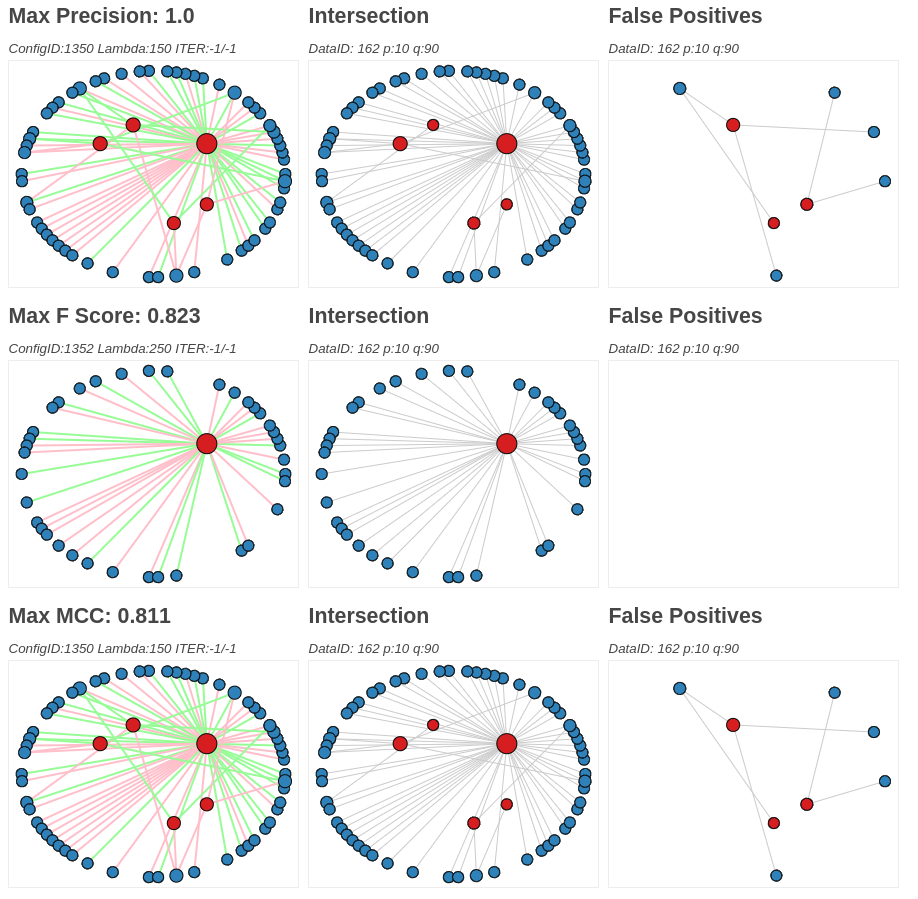
\includegraphics[width=1\linewidth]{graph_GLASSO_162}
	\caption{W12 subnetwork reconstructed with GLASSO(for artificial data set with id 162)}
	\label{fig:network_GLASSO162}
\end{figure}



